
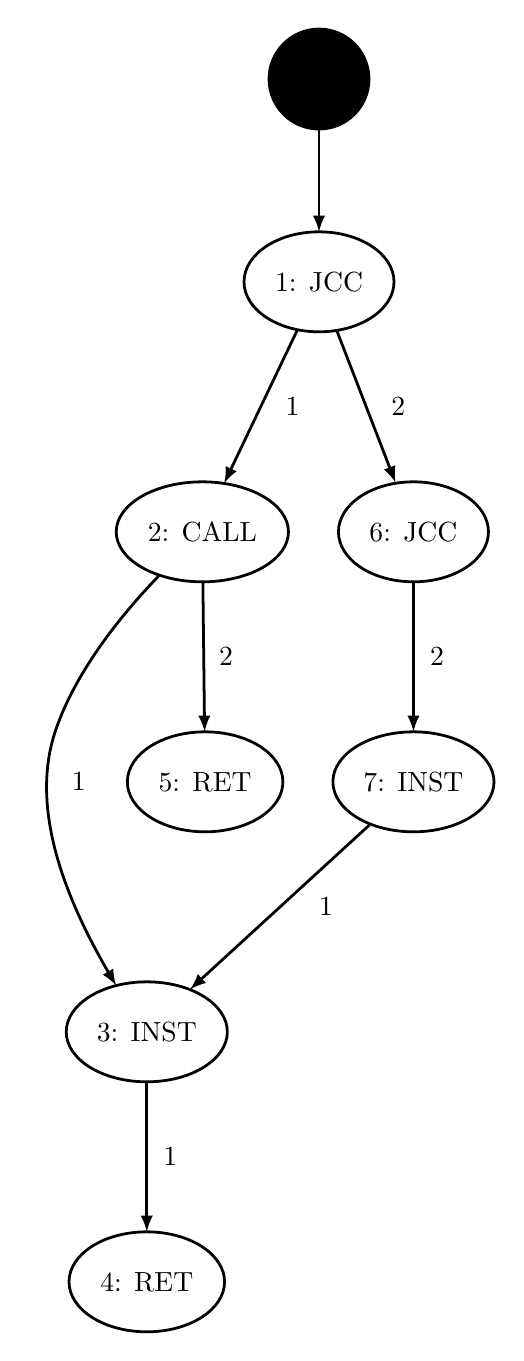
\begin{tikzpicture}[>=latex,line join=bevel,]
  \pgfsetlinewidth{1bp}
%%
\pgfsetcolor{black}
  % Edge: 2 -> 3
  \draw [->] (40.765bp,272.35bp) .. controls (27.923bp,259.06bp) and (10.62bp,238.19bp)  .. (3.2513bp,216.0bp) .. controls (-6.13bp,187.75bp) and (7.5181bp,155.01bp)  .. (25.211bp,124.66bp);
  \definecolor{strokecol}{rgb}{0.0,0.0,0.0};
  \pgfsetstrokecolor{strokecol}
  \draw (11.751bp,198.0bp) node {1};
  % Edge: 6 -> 7
  \draw [->] (132.25bp,269.61bp) .. controls (132.25bp,257.24bp) and (132.25bp,240.37bp)  .. (132.25bp,216.05bp);
  \draw (140.75bp,243.0bp) node {2};
  % Edge: 1 -> 6
  \draw [->] (104.65bp,360.45bp) .. controls (109.55bp,347.75bp) and (116.43bp,329.96bp)  .. (125.77bp,305.78bp);
  \draw (126.75bp,333.0bp) node {2};
  % Edge: 7 -> 3
  \draw [->] (116.4bp,182.47bp) .. controls (100.88bp,168.24bp) and (77.069bp,146.42bp)  .. (51.809bp,123.26bp);
  \draw (100.75bp,153.0bp) node {1};
  % Edge: 1 -> 2
  \draw [->] (90.351bp,360.45bp) .. controls (84.192bp,347.54bp) and (75.528bp,329.39bp)  .. (64.116bp,305.48bp);
  \draw (88.751bp,333.0bp) node {1};
  % Edge: 0 -> 1
  \draw [->] (98.251bp,432.81bp) .. controls (98.251bp,424.79bp) and (98.251bp,415.05bp)  .. (98.251bp,396.03bp);
  % Edge: 2 -> 5
  \draw [->] (56.449bp,269.61bp) .. controls (56.59bp,257.24bp) and (56.781bp,240.37bp)  .. (57.058bp,216.05bp);
  \draw (64.751bp,243.0bp) node {2};
  % Edge: 3 -> 4
  \draw [->] (36.251bp,89.614bp) .. controls (36.251bp,77.24bp) and (36.251bp,60.369bp)  .. (36.251bp,36.05bp);
  \draw (44.751bp,63.0bp) node {1};
  % Node: 1
\begin{scope}
  \definecolor{strokecol}{rgb}{0.0,0.0,0.0};
  \pgfsetstrokecolor{strokecol}
  \draw (98.25bp,378.0bp) ellipse (27.0bp and 18.0bp);
  \draw (98.251bp,378.0bp) node {1: JCC};
\end{scope}
  % Node: 0
\begin{scope}
  \definecolor{strokecol}{rgb}{0.0,0.0,0.0};
  \pgfsetstrokecolor{strokecol}
  \definecolor{fillcol}{rgb}{0.0,0.0,0.0};
  \pgfsetfillcolor{fillcol}
  \filldraw [opacity=1] (98.25bp,451.0bp) ellipse (18.0bp and 18.0bp);
\end{scope}
  % Node: 3
\begin{scope}
  \definecolor{strokecol}{rgb}{0.0,0.0,0.0};
  \pgfsetstrokecolor{strokecol}
  \draw (36.25bp,108.0bp) ellipse (29.0bp and 18.0bp);
  \draw (36.251bp,108.0bp) node {3: INST};
\end{scope}
  % Node: 2
\begin{scope}
  \definecolor{strokecol}{rgb}{0.0,0.0,0.0};
  \pgfsetstrokecolor{strokecol}
  \draw (56.25bp,288.0bp) ellipse (31.0bp and 18.0bp);
  \draw (56.251bp,288.0bp) node {2: CALL};
\end{scope}
  % Node: 5
\begin{scope}
  \definecolor{strokecol}{rgb}{0.0,0.0,0.0};
  \pgfsetstrokecolor{strokecol}
  \draw (57.25bp,198.0bp) ellipse (28.0bp and 18.0bp);
  \draw (57.251bp,198.0bp) node {5: RET};
\end{scope}
  % Node: 4
\begin{scope}
  \definecolor{strokecol}{rgb}{0.0,0.0,0.0};
  \pgfsetstrokecolor{strokecol}
  \draw (36.25bp,18.0bp) ellipse (28.0bp and 18.0bp);
  \draw (36.251bp,18.0bp) node {4: RET};
\end{scope}
  % Node: 7
\begin{scope}
  \definecolor{strokecol}{rgb}{0.0,0.0,0.0};
  \pgfsetstrokecolor{strokecol}
  \draw (132.25bp,198.0bp) ellipse (29.0bp and 18.0bp);
  \draw (132.25bp,198.0bp) node {7: INST};
\end{scope}
  % Node: 6
\begin{scope}
  \definecolor{strokecol}{rgb}{0.0,0.0,0.0};
  \pgfsetstrokecolor{strokecol}
  \draw (132.25bp,288.0bp) ellipse (27.0bp and 18.0bp);
  \draw (132.25bp,288.0bp) node {6: JCC};
\end{scope}
%
\end{tikzpicture}

